\documentclass{article}
\usepackage{hyperref}
\usepackage{graphicx}

\title{Dark-Sky Y790 Conclusions}
\author{Zack Marvel}
\date{\today}
\begin{document}
\maketitle

% MOTIVATION
\section*{Background}
The original motivation for the work I did this semester was the National Parks Service management of Hoosier National Forest seeking designation by the International Dark-Sky Association\footnote{\url{http://www.darksky.org/idsp/}}. The designation in the context of a park means the park has areas with a low level of light pollution; it requires updates from the designee to ensure that the level of light pollution in the area does not increase.

Through the course of the semester, Bryce relayed a conversation with an astronomer with the groups working on the project about how astronomers hoping to do some observation with a portable telescope typically look for such a location. We initially hoped we could provide a service useful to people with the Parks Service (for the purposes of the designation) \emph{and} astronomers wanting to use telescopes. It turns out that astronomers generally use a ``Clear Sky Chart\footnote{\url{http://www.cleardarksky.com/c/BlmngtnINkey.html?1}}'' (like Figure~\ref{fig:clear_sky_chart}) to look at a forecast over a couple days. The chart includes such factors as cloud cover and how dark the specified area is predicted to be.

% 
\begin{figure}[h]
  \centering
  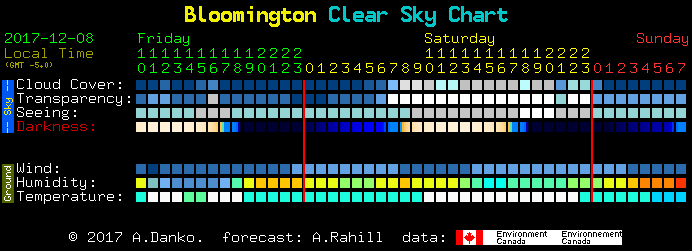
\includegraphics[scale=0.5]{bloomington_clear_sky_chart}
  \caption{Clear Sky Chart for Bloomington, IN} \label{fig:clear_sky_chart}
\end{figure}

A weather forecast can provide a cloud cover estimate. Satellite imagery\footnote{\url{http://www.cleardarksky.com/lp/BlmngtnINlp.html?Mn=equatorial\%20mount}} can be used to detect the amount of light pollution coming from an area, but the resolution is limited. Only with some kind of sensor on the ground can we hope to detect, for example, if somebody living near the edge of Hoosier National Forest has installed a new dusk-to-dawn light on their property, increasing the light pollution in the park itself.

Although a simple light sensor can tell us if an area of the park is brighter than expected, it can't tell us if it's dark because it's cloudy or because it's a dark, clear night. Consider that a cloudy night could actually be darker than a clear, starry night; or that a clear night with a full moon is not as useful since the moon dominates the sky. Also, certain areas of the sky could be of greater interest to astronomers than others. A light sensor alone cannot tell us which \emph{parts} of the sky are light-polluted. But perhaps the additional information could be useful to someone using a clear sky chart who has determined that Hoosier National Forest could be a good location for observation on a given date and wants to determine which areas of the park are darkest.

Ultimately, we chose to focus our work this semester on providing a solution to the problem faced by the Parks Service---for the Dark-Sky designation, they're required to perform continual monitoring. Unihedron\footnote{\url{http://www.unihedron.com/projects/darksky/}} produces a ``sky quality meter'' which estimates the amount of light pollution in an area by pointing it up at the sky. It just uses a light sensor internally and provides a value in magnitudes per arcseconds squared---apparent magnitude is the brightness of an object in space from the ground.

Unihedron produces a model of their sky quality meter with an ethernet port for uploading measurements to the Internet, but this meter is designed for locations with a constant Internet connection (ethernet port) and power supply. We wanted to find a solution that could be deployed with more flexibility and less maintenance. We set our sights on a solar-powered system with a cellular modem for uploading readings.

We met with the Parks Service people at the beginning of the semester, and they suggested some locations that should be pretty dark. Gianpaolo and I visited some of these locations with the Unihedron meter to confirm that they actually \emph{were} fairly dark, accessible, and there were no obvious sources of light pollution very nearby. In total, we visited five locations, and we were able to determine which ones were unlikely to have cellular service---since we planned to use a modem, this was a requirement in addition to darkness.

% NUCLEO PROTOTYPE
\section*{Prototype}
I prototyped the sensor with an STM32L476RG Nucleo-64 (like in Figure~\ref{fig:nucleo}). Unihedron's meter uses a TSL237 light sensor, made by TAOS. I had a light sensor from the same manufacturer with an I\textsuperscript{2}C interface, a TSL2561, lying around at home.

\begin{figure}[h]
  \centering
  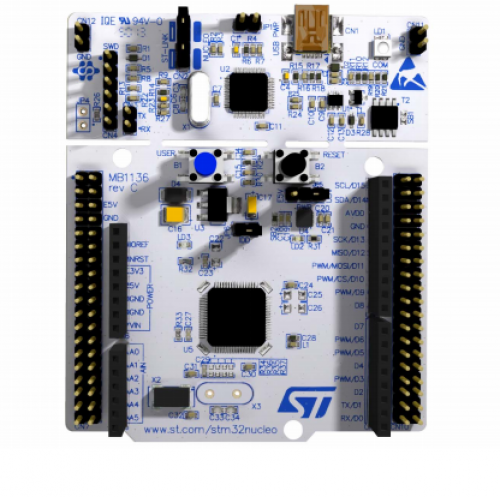
\includegraphics[scale=0.5]{nucleo_64_stm32f303re}
  \caption{STM32 Nucleo-64} \label{fig:nucleo}
\end{figure}

I designed a simple prototype that recorded the reading from the TSL2561 (seen in Figure~\ref{fig:tsl2561}) into flash. The STM32L476 should consume about 16 mW at 80 MHz in ``run'' mode; the light sensor should consume less than 1 mW. Even running constantly, with a commodity 10 Ah cell phone battery pack, we would expect about 80 days of uptime before the battery died.

\begin{figure}[h]
  \centering
  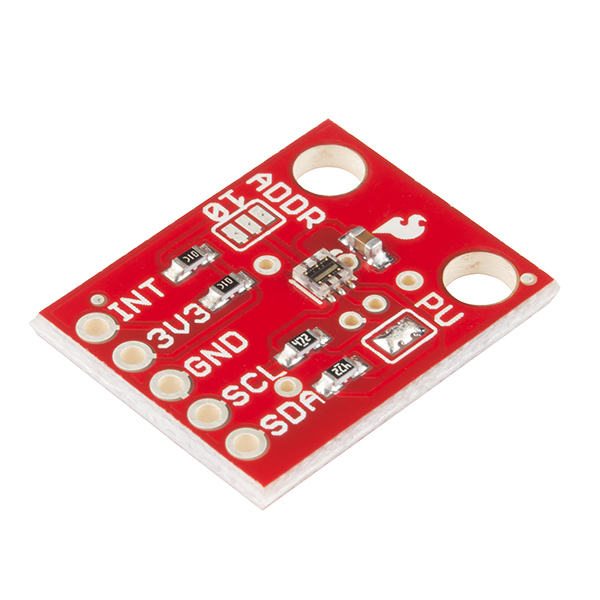
\includegraphics[scale=0.25]{sparkfun_tsl2561}
  \caption{Sparkfun TSL2561 breakout} \label{fig:tsl2561}
\end{figure}

Compared to the TSL2561, the TSL237 has no I\textsuperscript{2}C interface---it outputs a frequency representing the light intensity. I had based my previous prototype on ChibiOS\footnote{\url{http://chibios.org/dokuwiki/doku.php}}, an RTOS which provides a nice HAL around many of the STM32's features, as well as threading and other OS features. I switched from using the I\textsuperscript{2}C driver to the ICU driver for frequency measurement. Ultimately, the goal would be to replicate the 

This approach would be useful to collect data for a location over a period of time, albeit impractical since it requires retrieving the sensor and changing the battery; the latency to retrieve data is also much higher than using a modem. If I had a breakout for the modem we planned to use, I could have developed the prototype further. However, the goal of the class was to learn some hardware design, so I went ahead with designing a shield for the Nucleo-64 with a modem and light sensor onboard.

% PARTICLE ELECTRON
\section*{Shield Design}
The Particle Electron\footnote{\url{https://www.particle.io/products/hardware/electron-cellular-dev-kit}} (shown in Figure~\ref{fig:electron}) is a prototyping platform with a cellular modem based on the STM32F205. It has an Arduino-like software API (based on FreeRTOS\footnote{\url{https://www.freertos.org/}}) for rapid prototyping. Another student developed a prototype remote light sensor based on this system, and I based the modem part of my shield design on the Electron as well. Particle publishes their hardware designs (for Eagle) on Github, including those for the Electron\footnote{\url{https://github.com/spark/electron}}.

\begin{figure}[h]
  \centering
  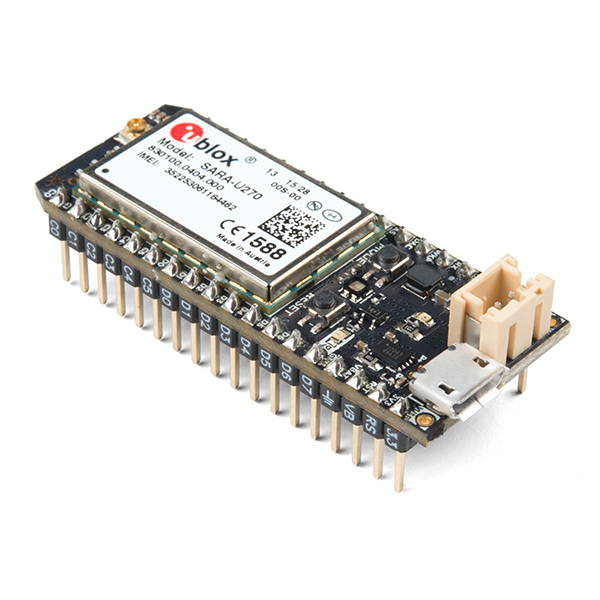
\includegraphics[scale=0.3]{particle_electron}
  \caption{Particle Electron} \label{fig:electron}
\end{figure}

% SHIELD DESIGN
I designed my shield in Kicad rather than Eagle. This meant I had to create several Kicad symbols for my schematic and some Kicad modules for my footprint from scratch. For example, though the level shifters and line drivers required for the modem were a standard footprint, the modem itself was not; designing its footprint was a good experience. In the case of the SIM card holder, I deviated from the nano-SIM on the Electron to a full-sized SIM because there was a footprint available in Kicad.

Some modifications to the Electron design were necessary. Primarily, the Electron has an onboard power management IC which converts the 5 V provided by the USB to 3.8 V for the modem, then converted down by a buck converter to 3.3 V for the STM32. In my case, the Nucleo has its own onboard regulator; the shield connector provides both 5 V and 3.3 V. I used a different buck converter to drop the voltage from 5 V to 3.8 V.

Concerns with this hardware implementation are that the modem could actually have current requirements that exceed the voltage regulator on the Nucleo. For example, the LD1117S50TR has a max output current of 1300 mA, and the LD39050PU33R has a min output current of 500 mA. The modem may consume up to 2 A under certain conditions, so using the Nucleo's voltage regulation hardware is likely to be unreliable. It would be pretty easy to add a USB port to the shield, which could use the current buck converter with no changes.

% NEXT STEPS
\section*{Next Steps}
The next step would be the fabrication and assembly of the actual shield design. After that, I could start writing software for it, either porting the Particle Electron firmware to the L476, or porting only parts of it (in particular the cellular modem driver) to some other firmware like my ChibiOS prototype. Ideally the cloud services provided by Particle would still be available with unofficial hardware, but if not it would be pretty trivial to design an API that could consume the sensor data.

The advantage to moving to the L4 core instead of the F2 is the architecture offers lower-power features, such as ``deep sleep'' modes which consume much less power than the low-power modes on the F2. The modem is the big power hog, but it can be powered off except to upload data once a day. The L476 must be able to read the light sensor intermittently throughought the night, but it can be in a low-power mode most of the time.

Finally, we'd like to deploy the sensors across Hoosier National Forest. Other students this semester worked on a web interface, so it would be possible to display light sensor readings over the course of a month, for example. It would be nice to send an email or display an alert if a light sensor detected an unusual amount of light. The web service could filter out full moon nights, for example, so Parks Service employees could be alerted about consistent excessive light readings, suggesting a light pollution source had been installed nearby. Ultimately, Hoosier National Forest would be able to attain the Dark-Sky designation.
\end{document}
